\documentclass{article}

\usepackage{enumerate}
\usepackage{enumitem}
\usepackage{mathtools}
\usepackage{amsmath, amssymb}
\usepackage{float}
\usepackage[margin=25mm, bottom=15mm]{geometry}
\usepackage{graphicx} % Required for inserting images
\usepackage{xurl}
\usepackage{xcolor}
\usepackage{wrapfig}
\usepackage{hyperref}
\usepackage{blindtext}
\usepackage{caption}
\usepackage{multicol}
\usepackage[
backend=biber,
style=ieee,
]{biblatex}
\hypersetup{
    colorlinks,
    citecolor = violet,
    filecolor = violet,
    linkcolor = violet,
    urlcolor = violet
}
\usepackage{listings}
\lstset{
    language = Python,
    tabsize = 2,
    showstringspaces = false,
    breaklines = true,
    basicstyle = \ttfamily,
    keywordstyle = \color[rgb]{0.1,0.3,0.7}\ttfamily,
    stringstyle = \color[rgb]{0.7,0.1,0.3}\ttfamily,
    commentstyle = \color[rgb]{0.3,0.4,0.3}\ttfamily,
    columns = fixed,
    numberstyle = \sffamily\scriptsize,
    backgroundcolor = \color[rgb]{0.95,0.95,0.95},
    frame = lines,
    framexleftmargin=5pt,
    numbers = left,
    numberstyle = \footnotesize
}
\numberwithin{figure}{section}  % Makes figure number match the section number
\numberwithin{equation}{section}  % Same thing but for equations
\addbibresource{references.bib}
\newcommand{\vect}[1]{\mathbf{#1}}

% Header up there
%%%%%%%%%%%%%%%%%%%%%%%%%%%%%%%%%%%%%%%%%%%%%%%%%%%%%%%%%%%%%%%
%%%%%%%%%%%%%%%%%%%%%%%%%%%%%%%%%%%%%%%%%%%%%%%%%%%%%%%%%%%%%%%
% Actual document down here

\title{Simulation of airflow through a window with an anti-bug grid}
\author{Martin Opat (s4704126), Robin Sachsenweger Ballantyne (s4617096)}
\date{November 2024}

\begin{document}

\maketitle



\section{Introduction}

\begin{wrapfigure}{r}{0.45\textwidth}
\vspace{-2cm}
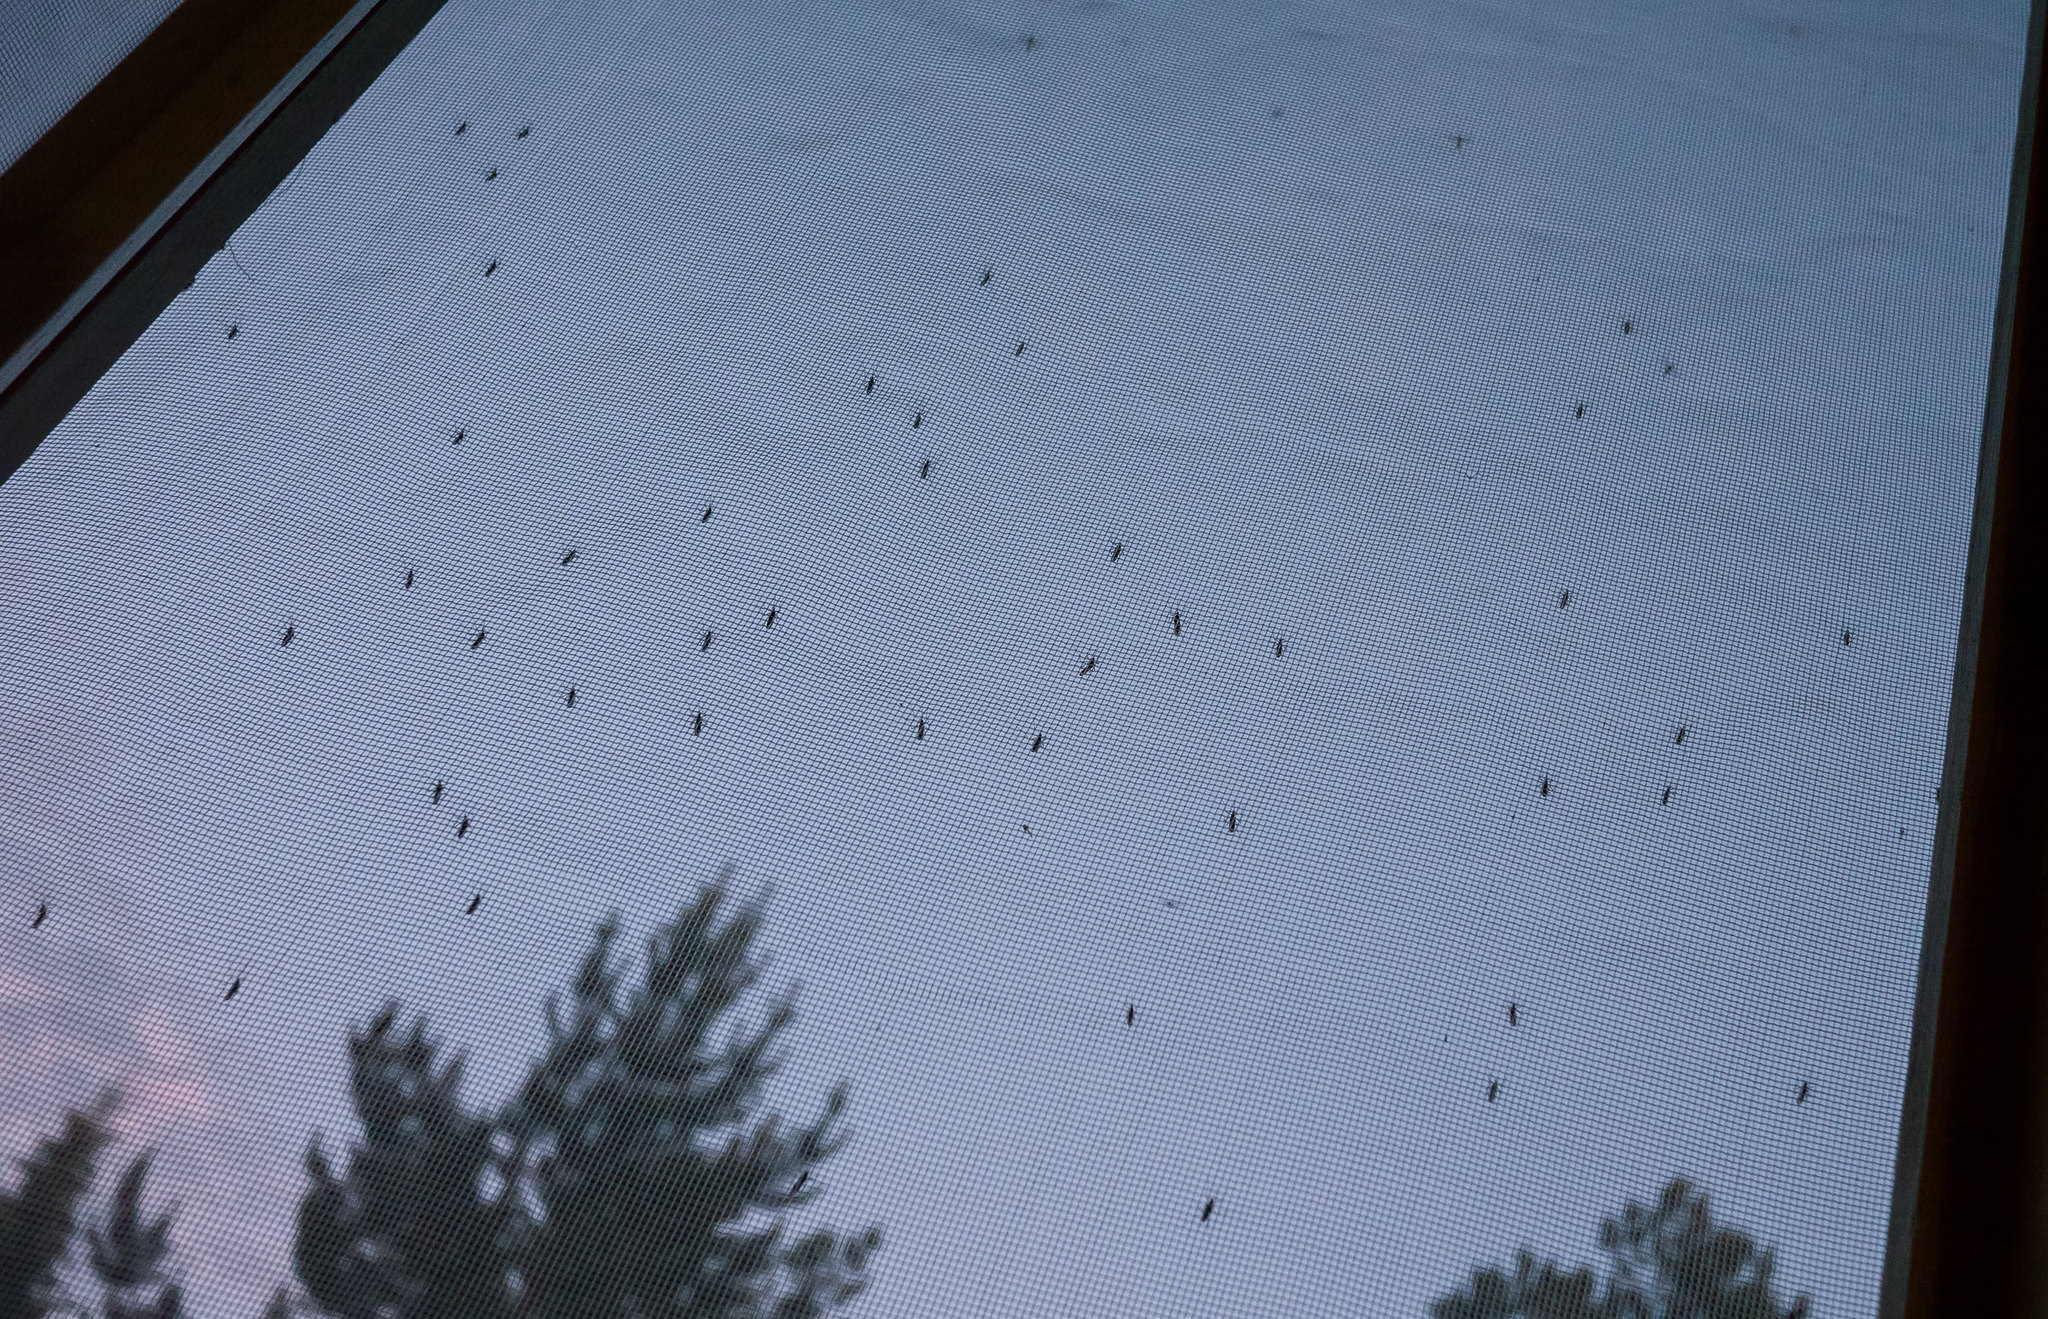
\includegraphics[width=0.9\linewidth]{figures/mosquitogrid.jpg}
\caption{Anti-bug grid (\href{https://www.flickr.com/photos/neekohfi/7817306994/}{Flickr.com})}\
\end{wrapfigure}

Bug grids can be placed over open windows to allow air to flow through without letting bugs into someone's house. Presumably, when people open their windows, they want air to flow through their house. However, our hypothesis is that a bug grid will decrease the flux and that different grids will affect the flux differently. Using a fluid flow simulation, we want to study how the grid's thickness and hole density affect the flux. Finding optimal thickness and hole density can help design anti-bug grids.

\subsection{Research question}
\textbf{Main:}
\begin{itemize}
    \item How much does the air flux through a window with a bug grid change with the grid's thickness and density?
\end{itemize}
\textbf{Subquestions:}
\begin{itemize}
    \item What are the optimal parameters of the grid that maximise airflow while keeping the bugs out?
    \item In which section of the window has the airflow decreased the most due to the presence of the bug grid?
\end{itemize}

\newpage


\section{Model and Methodology}
We aim to implement a numerical 3D simulation of airflow based on Navier-Stokes equations in Python. The numerical simulation will include discretising space and time. The cells that make up the bug grid will be modelled using a no-slip boundary condition.

\subsection{Assumptions:}
\begin{multicols}{2}
\begin{enumerate}
    \item Mass conservation
    \item Isotropy (i.e., no gravity)
    \item Compressible fluid
    \item Dynamic ($\mu$) and bulk ($\zeta$) viscosities are uniform in space
    \item Stoke's hypothesis ($\zeta=0$)
    \item Newtonian fluid
\end{enumerate}
\end{multicols}

\subsection{Math}
The assumptions above yield the Navier-Stokes equation(s) \cite{batchelor2000introduction} in the following form:
\begin{equation}
{\left(\partial_t +\mathbf {u} \cdot \nabla -\nu \,\nabla ^{2}-({\tfrac {1}{3}}\nu +\xi )\,\nabla (\nabla \cdot )\right)\mathbf {u} =-{\frac {1}{\rho }}\nabla p+\mathbf {f} ,}
\end{equation}

where $\rho$ is the mass density, $\vect{u}$ is velocity, $p$ is the pressure, $\nu$ is a shear kinematic viscosity parameter, $\xi$ is the bulk kinematic viscosity, and $\vect{f}$ is the body force (which is 0 due to isotropy).
Further "massaging" the equation:
\begin{gather}
    \partial_t \vect {u} + \underbrace{(\mathbf {u} \cdot \nabla) \vect {u} -\nu \,\nabla ^{2}\vect {u}-({\tfrac {1}{3}}\nu +\xi )\,\nabla (\nabla \cdot \vect {u})}_{f\left(\vect{u}\right)} =-{\frac {1}{\rho }}\nabla p,
\end{gather}
where $f(\vect{u})$ is a function of $\vect{u}$ and its spatial (partial) derivatives.
\begin{gather}
    % \partial_t \vect{u} + f(\vect{u}) = -{\frac {1}{\rho }}\nabla p \\
    \partial_t \vect{u}  = -f(\vect{u}) -{\frac {1}{\rho }}\nabla p \label{eq: NS-cont-final}
\end{gather}
Applying the finite difference method to the time derivative in eq. \ref{eq: NS-cont-final}, we get:
\begin{gather}
    \frac{\vect{u}_{ijk}^{n+1} - \vect{u}_{ijk}^n}{\Delta t} = -f(\vect{u}^n) -{\frac {1}{\rho }}\nabla p \\
    \vect{u}_{ijk}^{n+1} = \vect{u}_{ijk}^n - \Delta t \left(f(\vect{u}^n) + {\frac {1}{\rho }}\nabla p\right), \label{eq: NS-fd}
\end{gather}
where $\Delta t$ is the discrete time-step size, $n$ is the time-step index, and $i,j,~\text{and}~k$ are the indices in the $x,y,~\text{and}~z$ spatial coordinates respectively. We can apply the finite difference method to all the (spatial) derivatives in $f$ in the same way as we did above.

We also impose the no-slip boundary condition at the location of the rectangular bug grid, as well as on the walls around the window:
\begin{gather}
    \forall i,j,k \in [\text{grid},~\text{window}] ~\forall n:~ \vect{u}_{ijk}^n = \vect{0} \label{eq: boundary}
\end{gather}

\newpage

\section{Simulation setup}
There are two ways of approaching the numerical simulation of the equations above:
\begin{enumerate}
    \item Giving eq. (\ref{eq: NS-cont-final}) into a PDE solver
    \item Implement and perform a numerical integration using eq. (\ref{eq: NS-fd})
\end{enumerate}
Option 1. is the preferred option, assuming a PDE-solve Python package exists that can accommodate eqs. (\ref{eq: NS-fd}) and (\ref{eq: boundary}). Option 2. is a backup option, and will only be used if no existing package fits our criteria well enough.



% % TODO: Add simulation details
% % TODO: Add simulation output + postprocessing description

% \section{Planning}
% The planning of the project is split below into discrete chronological bullet points:
% \begin{itemize}
%     \item Look for an existing, suitable PDE solver Python package. If such a package is found, read the documentation and get a simple example working to test its suitability; otherwise, research numerical integration schemes that will fit our case. \textbf{[1 Week]}
%     \item Implement the simulation \textbf{[2 Weeks]}
%     \item Run the simulation with different parameter values and export the simulated data (text format)
%     $\rightarrow$ process the data, i.e., plot the relevant graphs (e.g., flow vs grid density) and figures. \textbf{[2 Weeks]}
%     \item Discuss the results. \textbf{[1 Week]}
% \end{itemize}

\newpage

\section{Results}

\newpage
\section{Discussion}

\newpage
\section{Conclusion}
\newpage

\printbibliography

\end{document}
